\Chapter{Tervezés}


\Section{Felhasznált technológiák}


\SubSection{C\#}

Az egyetemi éveim alatt lehetőségem volt 2 féléven keresztül az evosoft Hungary Kft. evoCampus-án részt venni, ahol megismerkedtem a C\# nyelvvel, amelyet végül az alkalmazásom megvalósításához választottam.

A C\# egy általános célú, objektumorientált programozási nyelv, valamint a .NET egyik fő programozási nyelve. A C nyelvcsaládhoz tartozik, így ismert lehet a C++ és Java programozók számára, hiszen ilyen alapokon fejlesztették ki. Platformfüggetlenségét a .NET környezet biztosítja.

A .NET keretrendszer gyors és hatékony alkalmazásfejlesztést biztosít a .NET osztálykönyvtárak által. A különböző nyelveken írt komponensek együttműködését pedig a CLR (Common Language Runtime) és a CTS (Common Type Sytem) segítségével könnyíti meg.

% TODO: hivatkozás

\SubSection{Visual Studio}

A Visual Studio egy integrált fejlesztői környezet, amelyet a Microsoft fejlesztett ki különböző alkalmazások, pl.: konzol, webalkalmazások, mobilalkalmazások fejlesztésére. Lehetőséget nyújt a C\#-on kívül például Viusal Basic, F\# és számos más nyelveken történő programozásra.  Az alkalmazásom megvalósításakor én a Community kiadást választottam, ami egy olyan ingyenes verzió, amely a Professional kiadáshoz hasonló szolgáltatásokat tartalmaz.

% TODO: hivatkozás

\SubSection{WPF}

A WPF (Windows Presentation Foundation) egy grafikus felhasználói felületet biztosító keretrendszer. Előnye a XAML nyelv, amely megkönnyíti a felhasználói felület létrehozását és szerkesztését, valamint lehetővé teszi magának a UI tervezésének elkülönítését a program többi részétől. Emellett, lehetőség van DataBinding használatára, amely állandó kapcsolatot biztosít az alkalmazás felhasználói felülete és backend-en tárolt adatok között. Így, egy adat backend-en történő értékének megváltozása során a felhasználói felület automatikusan fog frissülni és fordítva.

% TODO: hivatkozás

\SubSection{MVVM}
Az MVVM rövidítés a Model, View, ViewModel szavakból származik. A séma lényege, hogy az alkalmazásunkat erre a három, jól elkülöníthető logikai egységre szedjük szét, mely által jobban átláthatóvá válnak. A három egység különböző célokat szolgál.

\begin{figure}[h]
	\centering
	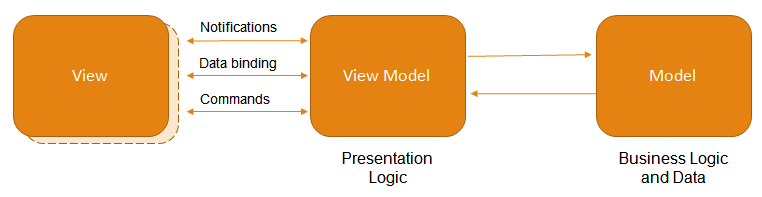
\includegraphics[scale=0.5]{images/mvvm.png}
	\caption{Az MVVM működése}
	\label{fig:mvvm}
\end{figure}

% TODO: kép, hivatkozás

A View szerepe a grafikus felület biztosítása, minden, amit a képernyőn meg szeretnénk jeleníteni, azt megadhatjuk itt a XAML kód által. A XAML kódon belül definiáljuk a binding-okat is.

A Model tartalmazza a különböző adatokat és osztályokat, amikkel dolgozni szeretnénk.

A ViewModel pedig a kettő közötti kapcsolatot adja meg. Itt történik például a példányosítás, és ezáltal jeleníthetjük meg azt, amit a View-n látni szeretnénk, általában command-okon keresztül.
% TODO: hivatkozás

\SubSection{Azure DevOps}

Az Azure DevOps (korábban Visual Studio Team Foundation Server (TFS)) fejlesztői szolgáltatásokat nyújt csapatok számára a munka megtervezéséhez, a kódfejlesztésben való együttműködéshez, valamint alkalmazások készítéséhez és telepítéséhez. Én személy szerint a verziókövetés miatt tartottam fontosnak a használatát, mivel lehetővé teszi, hogy a kódban történő változtatásokat nyomon követhessem, engedélyezi, hogy szükség esetén egy korábbi változatra visszaálljak és nyilvántartja a különbségeket a verziók között. Különböző verziókat is összeilleszthetünk, ilyenkor a módosítások miatt felmerülő problémák esetén pedig a konfliktusok lekezelésére is lehetőség van.

\begin{figure}[h]
	\centering
	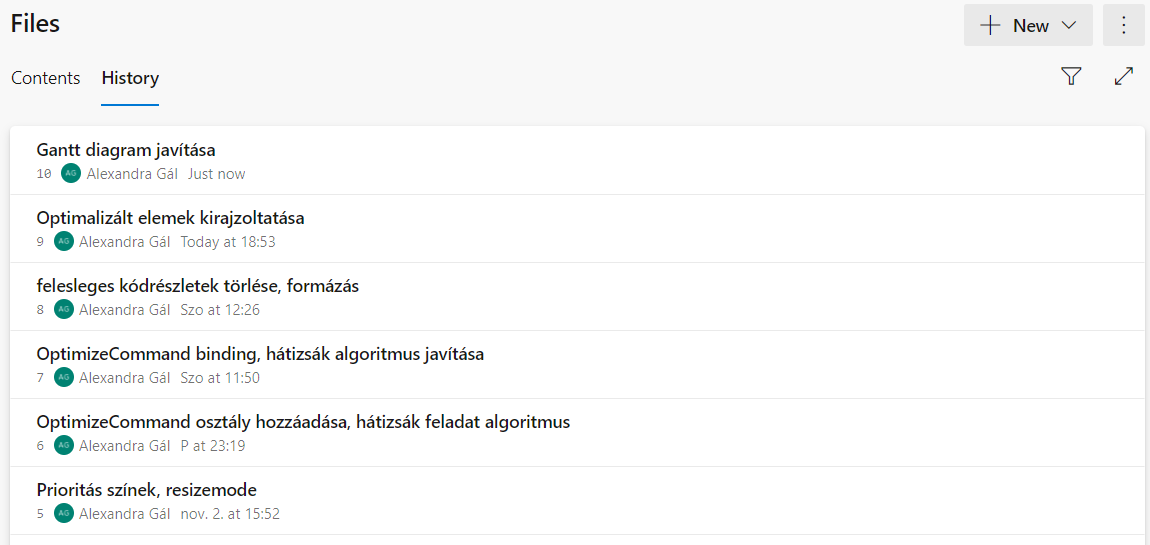
\includegraphics[scale=0.5]{images/azureHistory.png}
	\caption{Verziókövetés az Azure DevOps-ban}
	\label{fig:azure}
\end{figure}

\SubSection{ItemsControl, Canvas, Rectangle osztály}

Mivel C\#-ban a legtöbb lehetőség a diagramokat illetően a WinForms-hoz kapcsolódik és nem a WPF-hez, vagy pedig nem nyílt forráskódú könyvtárak által lenne lehetséges, ezért úgy döntöttem, hogy a vizuális ábrázolást az ItemsControl, a Canvas, és a Shape könyvtár közül a Rectangle osztály segítségével oldom meg.

A Rectangle osztály segít a téglalapok megrajzolásában, ami a feladatok hosszát reprezentáló sávot ábrázolja majd a diagramon.

A Canvas egy olyan területet biztosít, ahol elemeket tudunk pozícionálni.

Az ItemsControl fogja tartalmi a Canvast, amelyet az ItemsControl ItemsPanel-jére tudunk elhelyezni. Az ItemsControl-ra azért van szükség, mert a kirajzolandó téglalapok egy Rectangle típusú ObservableCollection-ben lesznek eltárolva és ez a Control a kollekciók elemeinek megjelenítését segíti.




\Section{UML diagram}

% TODO: Tervezett osztályok, UML osztálydiagram. (Komponenseken belüli részek, metódus szignatúrák.)



\Section{Adatmodell}

% TODO: Áttekintő blokkdiagram, például, hogy az alkalmazás egyes részei hogyan kapcsolódnak egymáshoz (komponensek, interfészek).

% ezeket a részeket nem tudom pontosan hogy kéne megírni
